\section{Background}
\label{sec:background}

\subsection{Blockchain and Tangle (DAG)}
Blockchain DLT become widely known in 2009 with the launch of Bitcoin network. 
Participants in the network can validate and verify the transactions independently, without relying on central trust parties. 
Blockchain is usually maintained and managed by a distributed group of participants independently. 
This along with its cryptographic mechanisms ensures the data recorded on the ledger immutable \cite{Yaga2018BlockchainTO}. 
The structure of a traditional blockchain can be simplified as a singly linked list\footnote{Singly linked list: linked list which is unidirectional and can only be traversed on one direction.}, 
you can traverse from the latest block to the Genesis block\footnote{Genesis block: the first block of a blockchain. It is a special case as it does not reference a previous block.} (as shown in figure~\ref{fig:blockchain_structure}). 
Transactions are hashed in a Merkle Tree \cite{merkle1980protocols} for saving storage space and simplifying transaction validation. 


\begin{figure}[h]
    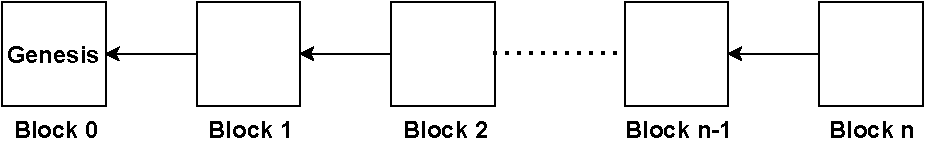
\includegraphics[width=0.45\textwidth,trim={-2cm -1cm 0 -1cm},clip]{figs/blockchain_structure.pdf}
    \caption{Blockchain structure}
    \label{fig:blockchain_structure}
\end{figure}


In the original Bitcoin whitepaper \cite{nakamoto2008peer}, Satoshi Nakamoto has listed the procedures for handling the transactions and record them on the blockchain ledger. 
All the nodes listen to the transactions broadcast to the network and each node collects new transactions for generating a new block. 
Then each node will do proof-of-work and broadcast the block to the network once it finds the solution for other nodes' validation. 
However, in real case, almost all the transaction wrapping and PoW are finished by specific miners in the network. Miners also require transaction fees for the reward of doing these.
The increasing of PoW complexity makes it nearly impossible to gain profit from mining Bitcoin with general PC hardware. Instead, dedicated miners have to use equipments like ASIC\footnote{ASIC: application-specific integrated circuit. It is the integrated circuit designed for a specific use case. Bitcoin ASIC chip can only handle computing tasks for Bitcoin mining, and cannot be used for any other tasks.} devoted specifically for the mining algorithm.
It is a potential hazard that the blockchain network will be centralized and controlled by the parties that owns most of the "mining rigs". In addition, blockchains relying on PoW are consuming massive energy \cite{sedlmeir2020energy}. According to CBECI\footnote{CBECI: Cambridge Bitcoin Electricity Consumption Index. Website: https://cbeci.org/}, Bitcoin network consumes approximately 130.51 TWh electricity per year, which is far more than the annual electricity consumption of some countries like Ukraine and Argentina. Carbon dioxide emission caused by these PoW blockchains will cause environmental issues like global warming.

\begin{figure*}[t]
    \centering
    \caption{Tangle structure}
    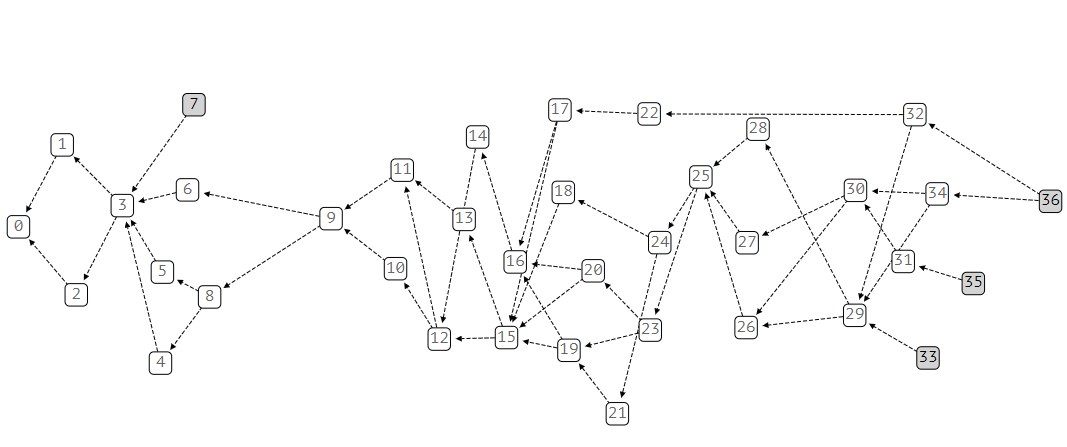
\includegraphics[width=\textwidth,trim={-1cm 0 0 0},clip]{figs/tangle_structure.png}
    \label{fig:tangle_structure}
\end{figure*}

Transaction throughput and transaction confirmation latency are two most critical performance issues about blockchain technology \cite{zhou2020solutions}. 
Transactions can only be recorded on the blockchain in sequence due to its linear structure. Also the limitation of size of each block makes it struggling to handle the enormous volume of transactions nowadays.
Blockchains including Bitcoin and Ethereum are facing problems like low TPS and bad scalability which results in transaction backlog and high transaction fees. 
In order to tackle these issues, people have put forward many alternative solutions such as side-chain, cross-chain, improved consensus, sharding, DAG, etc. 
IOTA Tangle is a new type of DLT addressing solving the problems above for IoT services. It has following advantages comparing with traditional blockchain technologies:

\begin{enumerate}
    \item \textbf{High scalability}. Directed-acyclic-graph structured Tangle ledger enables its high scalability. Serguei Popov has analyze the performances of the system under two different regimes: low load and high load in the article \textit{The Tangle} \cite{popov2018tangle}. In high load regime when more new tips\footnote{Tip: every new (unconfirmed) transaction is known as a tip.} are attached to Tangle, the typical time of a tip being approved is reduced. 
    So the larger the scale of the network, the more efficient it will be.
    \item \textbf{Feeless \& Environmental Friendly}. In DLT network like Bitcoin, we need to pay transaction fees to the miners for rewarding them wrapping our transactions to the block and conducting PoW computations. Transaction fees are considered part of the incentive for nodes to support the network. In IOTA Tangle, however, PoW consensus and miners are removed \cite{popov2019iota}. So it is more economical and environmental Friendly to use Tangle for sending transactions.
    \item \textbf{Quantum Computation Resistance}. IOTA Tangle uses post-quantum cryptography for securing data on the ledger \cite{tennant2017improving}. For instance, IOTA uses Winternitz One-Time Signature (WOTS), which is promising to be resistant to quantum computers \cite{buchmann2008post}. as a signature scheme protocol.
    \item \textbf{Lightweight}. IOTA node applications like GoHornet\footnote{GoHornet: IOTA full node software built in Go. Github source code: https://github.com/gohornet/hornet} is lightweight and can be easily installed and run on low-end devices such as Raspberry Pi 4.
\end{enumerate}

These characteristics are very crucial for IoT applications and favorable for building this project.


\subsection{Decentralized Naming System}
Before distributed ledger technology came into being, 

\subsection{P2P Network}


